\begin{frame}
\frametitle{Area of Interest in Bavaria}
\includegraphics[width=\textwidth]{images/aoi}
%\tikzstyle{annotation} = [fill=tumgraylight, rounded corners]

\tikzset{pic shift/.store in=\shiftcoord,
	pic shift={(0,0)},
	tcube/.pic = {
		%%% small temporal cube showing multitemporal observations %%%
		
		\begin{scope}[perspective3d, node distance=.8em]
			
			\def\size{3em}
			\def\d{.3}
			
			\node[fill=tumwhite, transform shape, canvas is yx plane at z=0*\d] (bottom) {\includegraphics[width=\size,height=\size]{images/tiles480/20160212}};
			\node[right=of bottom.east]{$t_{4}$};
			
			\node[fill=tumwhite, transform shape, canvas is yx plane at z=1*\d] (mid1) {\includegraphics[width=\size,height=\size]{images/tiles480/20160522}};
			\node[right=of mid1.east]{$t_{15}$};
			
			\node[fill=tumwhite, transform shape, canvas is yx plane at z=2*\d] (mid2) {\includegraphics[width=\size,height=\size]{images/tiles480/20160628}};
			\node[right=of mid2.east]{$t_{19}$};
			
			\node[fill=tumwhite, transform shape, canvas is yx plane at z=3*\d] (mid3) {\includegraphics[width=\size,height=\size]{images/tiles480/20160820}};
			\node[right=of mid3.east]{$t_{28}$};
			
			\node[fill=tumwhite, transform shape, canvas is yx plane at z=4*\d] (top) {\includegraphics[width=\size,height=\size]{images/tiles480/20160912}};
			\node[right=of top.east]{$t_{32}$};
			
			%\foreach \i in {south west, south east, north east, north west}
			%\draw[dashed] (bottom.\i) -- (top.\i) coordinate(b-\i);
			
			%\draw (b-south west)--(b-south east)--(b-north east)--(b-north west)--cycle;
			
		\end{scope}
	}
}
\tikzset{pic shift/.store in=\shiftcoord,
	pic shift={(0,0)},
	cube/.pic = {
	\begin{scope}[perspective3d]
		
		\def\cubewidth{13em}
		\def\d{.4}
		
		\node[canvas is yx plane at z=0*\d, draw, transform shape] (a) {\includegraphics[width=\cubewidth]{images/aoi/backgroundS2A20160721}};
		\node[canvas is yx plane at z=0*\d, transform shape, fill opacity=.2]{\resizebox{\cubewidth}{!}{\input{images/aoi/zoomed_gridtraintest.tikz}}};
		\node[canvas is yx plane at z=1*\d,draw,transform shape, fill opacity=1]{\resizebox{\cubewidth}{!}{\input{images/aoi/zoomed_480tiles.tikz}}};
		\node[canvas is yx plane at z=2*\d, draw,transform shape, opacity=1]{\resizebox{\cubewidth}{!}{\input{images/aoi/fields.tikz}}};
		
		%		\foreach \i in {south west, south east, north east, north west}
		%		\draw[dashed] (a.\i) --++(0,0,3) coordinate(b-\i);
		%		
		%		\draw (b-south west)--(b-south east)--(b-north east)--(b-north west)--cycle;
		%		
	\end{scope}
	}
}

\tikzset{pic shift/.store in=\shiftcoord,
	pic shift={(0,0)},
	map/.pic = {
	\begin{scope}[y=0.80pt, x=0.80pt, yscale=-0.15, xscale=0.15, inner sep=0pt, outer sep=0pt]
		
		
		\begin{scope}[cm={{0.99907,0.0,0.0,0.99907,(0.0,0.0)}},draw=black!30,line join=bevel,line cap=rect,line width=0.5pt]
			\input{images/aoi/borders.tikz}
		\end{scope}
		
		\begin{scope}[cm={{0.99907,0.0,0.0,0.99907,(0.0,0.0)}},draw=tumbluelight, fill=tumbluelight,line join=bevel,line cap=rect,line width=0.5pt]
			\input{images/aoi/germany.tikz}
		\end{scope}
		
%		\begin{scope}[cm={{0.99907,0.0,0.0,0.99907,(0.0,0.0)}},draw=tumblack,fill=tumblack,line join=bevel,line cap=rect,line width=0.5pt]
%			\input{images/aoi/aoibox.tikz}
%		\end{scope}
		
	\end{scope}
	}
}

\tikzset{pic shift/.store in=\shiftcoord,
	pic shift={(0,0)},
	zoomed/.pic = {
		\begin{scope}[]
			
			\def\boxwidth{13em}
			%\def\d{.4}
			
			\node[] (a) {\includegraphics[width=\boxwidth]{images/aoi/backgroundS2A20160721}};
			\node[fill opacity=.2]{\resizebox{\boxwidth}{!}{\input{images/aoi/zoomed_gridtraintest.tikz}}};
			\node[opacity=1]{\resizebox{\boxwidth}{!}{\input{images/aoi/buffered_tiles.tikz}}};
			%\node[fill opacity=1]{\resizebox{\cubewidth}{!}{\input{images/aoi/zoomed_480tiles.tikz}}};
			\node[opacity=1]{\resizebox{\boxwidth}{!}{\input{images/aoi/fields.tikz}}};
			
			%		\foreach \i in {south west, south east, north east, north west}
			%		\draw[dashed] (a.\i) --++(0,0,3) coordinate(b-\i);
			%		
			%		\draw (b-south west)--(b-south east)--(b-north east)--(b-north west)--cycle;
			%		
		\end{scope}
	}
}
%\tikzset{external/export next=false}
%\tikzsetnextfilename{aoimap}
\begin{tikzpicture}[]

%\node[](aoi) at (0,0){
%	%\begin{tikzpicture}[y=0.80pt, x=0.80pt, yscale=-0.15, xscale=0.15, inner sep=0pt, outer sep=0pt]
%	\begin{scope}[y=0.80pt, x=0.80pt, yscale=-0.15, xscale=0.15, inner sep=0pt, outer sep=0pt]
%	
%	
%	\begin{scope}[cm={{0.99907,0.0,0.0,0.99907,(0.0,0.0)}},draw=black!30,line join=bevel,line cap=rect,line width=0.5pt]
%	\input{images/aoi/borders.tikz}
%	\end{scope}
%	
%	\begin{scope}[cm={{0.99907,0.0,0.0,0.99907,(0.0,0.0)}},draw=tumbluelight, fill=tumbluelight,line join=bevel,line cap=rect,line width=0.5pt]
%	\input{images/aoi/germany.tikz}
%	\end{scope}
%	
%	\begin{scope}[cm={{0.99907,0.0,0.0,0.99907,(0.0,0.0)}},draw=tumblack,fill=tumblack,line join=bevel,line cap=rect,line width=0.5pt]
%	\input{images/aoi/aoibox.tikz}
%	\end{scope}
%	
%	\end{scope}
%	};

\coordinate (map) at (0,0);
\draw pic (aoi) at (map) {map};

%\draw[step=1.0,black,thin] (0,0) grid (5,-5);
\node[rectangle, inner sep=0, minimum width=4.5mm, minimum height=2mm, fill=tumblack, opacity=1] (aoirect) at ($ (map)+(2.15,-3.29) $){};

\coordinate (Berlin) at ($ (map)+(2.4,-1.3) $);
\node[annotation, above right= 5mm of Berlin](annotBerlin){\tiny Berlin};
\draw (Berlin) -- (annotBerlin);

\coordinate (Munich) at ($ (map)+(2.02,-3.45) $);
\node[annotation, below left= 5mm of Munich](annotMunich){\tiny Munich};
\draw (Munich) -- (annotMunich);

% draw relative to aoi node
%\begin{scope}[x={(aoi.south east)},y={(aoi.north west)}]
%\draw[red,ultra thick,rounded corners] (.5,.2) rectangle ++(0,0);
%\end{scope}

\visible<2->{
	\coordinate (A) at (6,-2);
	\node[inner sep=0](fold) at (A){
		\phantom{\resizebox{5cm}{!}{\input{images/aoi/fold0_with_margin.tikz}}}
	};	
	
	\draw (aoirect.south east) -- (fold.south east); 
	\draw (aoirect.south west) -- (fold.south west);
	\draw (aoirect.north east) -- (fold.north east);
	\draw (aoirect.north west) -- (fold.north west);
	
	\node[inner sep=0](fold) at (A){
		\resizebox{5cm}{!}{\input{images/aoi/fold0_with_margin.tikz}}
	};	
	
	\node[rectangle, inner sep=0, minimum width=4mm, minimum height=3mm, fill=tumblack, draw=tumblack, opacity=1] (foldrect) at ($ (fold)+(1,-.5) $){};
	
	\node[below = 1mm of fold](aoiwidth){\tiny \SI{102}{\km}};
	\node[left = 1mm of fold, anchor=center, rotate=90](aiuheight){\tiny \SI{40}{\km}};
	
	\coordinate (training) at ($ (A)+(-2,1.3) $);
	\node[annotation, fill=traincolor!40](annotTrain) at (training){\tiny training};
	\node[annotation, right= 3mm of annotTrain, fill=validcolor, text=white](annotValid){\tiny validation};
	\node[annotation, right= 3mm of annotValid, fill=evalcolor!40](annotEval){\tiny evaluation};

	\node[annotation](annotBlock) at ($ (A)+(3,-1.5) $){\tiny \SI{3840}{\m} blocks (14 \SI{240}{\m} tiles, \SI{480}{\m} margin)};
	
	\draw (annotBlock) -- ($ (A)+(1.52,-.9) $);
}

\visible<3->{
	\coordinate (B) at (11,-1);
	\draw[draw=white, double=black] (annotBlock) -- ($ (B)+(-.5,-.6) $);
	%\draw pic (bigcube) at (0,7,1.5) {zoomed};
	\phantom{\node[inner sep=0] (bigcube) at (B) {\includegraphics[width=4cm]{images/aoi/zoomed.pdf}};}
	%\draw pic (smallcube) at (0,10.5,2) {tcube};
	
	
	\draw (foldrect.south east) -- (bigcube.south east); 
	\draw (foldrect.south west) -- (bigcube.south west);
	\draw (foldrect.north east) -- (bigcube.north east);
	\draw (foldrect.north west) -- (bigcube.north west);
	
	\node[inner sep=0] (bigcube) at (B) {\includegraphics[width=4cm]{images/aoi/zoomed.pdf}};
	
	\coordinate (tileCoord) at ($ (B)+(.98,1.25) $);
	\node[annotation, above left=5mm of tileCoord](tileAnnot){\tiny tile (\SI{240}{\m})};
	\draw[black] (tileAnnot) -- (tileCoord); 
	
	\coordinate (marginCoord) at ($ (B)+(.6,-1.3) $);
	\node[annotation, below right=5mm of marginCoord](marginAnnot){\tiny margin (\SI{480}{\m})};
	\draw[black] (marginAnnot) -- (marginCoord); 
}



\end{tikzpicture}
\end{frame}


{\setbeamercolor{background canvas}{bg=black}
	\begin{frame}[plain]
	
	\vfill
	\Huge\color{white}
	\begin{center}
		\begin{columns}
			\column{.5\textwidth}
			\vspace{7em}
			
			\hfill 
			Earth Observation Data
			\column{.5\textwidth}
			
			\includegraphics[width=5cm]{images/epic1}
			%\includegraphics[width=7cm]{images/fdl}
		\end{columns}
	\end{center}
	
	\vfill
\end{frame}
}

\begin{frame}
\frametitle{System Earth}

\begin{columns}

\column{.5\textwidth}

{
	%		The Earth is a complex system.
	%		Only some components is observable by 
	%		\begin{itemize}
	%			\item satellite-based or
	%			\item in-situ observations
	%		\end{itemize}
	%		
	
	%	\begin{equation*}\V{y} = f({\M{X}})\end{equation*}
	%	partially observe the complex system Earth
	\textbf{Partially measuring} System Earth
	{\Huge
		\begin{center}
			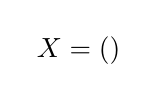
\begin{tikzpicture}[remember picture]
			\node[draw=none, rounded corners](eo){$\M{X} = \sat\left({\earth}\right)$};
			\end{tikzpicture}
		\end{center}
	}
	
	\vspace{1em}
	\textbf{knowledge extraction} through pattern recognition and machine learning
	
	{\Huge
		\begin{center}
			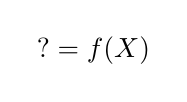
\begin{tikzpicture}[remember picture]
			\node[draw=none, rounded corners](ml){$\V{?} = f({\M{X}})$};
			\end{tikzpicture}
		\end{center}
	}
	
}

\column{.5\textwidth}

\begin{tikzpicture}[xscale=3, yscale=2]
\node(earth) at (0,0) {\includegraphics[width=7cm]{images/epicw1}};	

\end{tikzpicture}




\end{columns}


\begin{tikzpicture}[remember picture,overlay]
%\draw (0,1) to[grid with coordinates] (10,7);
\visible<2->{
\node[fill=tumbluedark, text=white, font=\Large, rounded corners](annoteo) at (7,6){Earth Observation Research};
\draw[annot] (annoteo.west)  to[bend right] (sat);
}

\visible<3->{
\node[fill=tumbluedark, text=white, font=\Large, rounded corners](annotml) at (7,3.5){Machine Learning Research};
\draw[annot] (annotml.west)  to[bend right] (ml);
}

\end{tikzpicture}


\end{frame}

\begin{frame}
\frametitle{Going Big...}

\includegraphics[width=5cm]{images/EuroCrops}
\includegraphics[width=5cm]{images/France}
\includegraphics[width=4cm]{images/Bavaria}

\end{frame}

\begin{frame}
\frametitle{Supported by Google Research Credits}

\includegraphics[width=.3\textwidth]{images/google_research_credits}
\includegraphics[width=.3\textwidth]{images/google}
\includegraphics[width=.2\textwidth]{images/earth-engine-logo}
%\includegraphics[width=3cm]{images/250px-Google-Cloud-Storage-Logo}
%\includegraphics[width=3cm]{images/Google_Compute_Engine_logo}
%\includegraphics[width=3cm]{images/google_cloud_sql}


\end{frame}


\begin{frame}
\frametitle{Augmenting Classification Models}

\begin{columns}
	
	\column{.5\textwidth}
	\begin{center}
		
		\input{images/backprop_example.tikz}
	\end{center}
	\column{.5\textwidth}
	\input{images/qualitative_example.tikz}
	
	
\end{columns}

\end{frame}


%\begin{frame}
%	\frametitle{Autoregressive Classification Model}
%	
%	\input{images/classmodel.tikz}
%	
%\end{frame}


\begin{frame}
\frametitle{Early Classification on Remote Sensing Data}
\input{images/example.tikz}

\url{https://arxiv.org/abs/1901.10681}


\end{frame}


\begin{frame}
\frametitle{Multi-Layer RNN baseline}

\input{images/confmat.tikz}

\begin{columns}
	
	\column{.5\textwidth}
	\textbf{Precision}
	
	\confmat{images/data/BreizhCrops_rnn/npy/confmat_flat.csv}{3}{1}
	
	\column{.5\textwidth}
	\textbf{Recall}
	
	\confmat{images/data/BreizhCrops_rnn/npy/confmat_flat.csv}{4}{1}
	
\end{columns}

\end{frame}

\begin{frame}
\frametitle{Transformer baseline}

\input{images/confmat.tikz}

\begin{columns}

\column{.5\textwidth}
\confmat{images/data/BreizhCrops_transformer/npy/confmat_flat.csv}{3}{1}

\column{.5\textwidth}
\confmat{images/data/BreizhCrops_transformer/npy/confmat_flat.csv}{4}{1}

\end{columns}

\end{frame}

